\documentclass[10pt,xcolor={usenames,dvipsnames,table}]{beamer}
\usepackage{tri_preamble}

%----------------------------------------------------------------------------------------
%	TITLE PAGE
%----------------------------------------------------------------------------------------

\title[Title]{Diffusion Models and Score Matching methods} 

\author{Tri Nguyen} 
\institute[OSU] 
{
Internal reading group \\
Oregon State University 
% \medskip
% \textit{nguyetr9@oregonstate.edu \endgraf } 
% }
}
\date{\today} % Date, can be changed to a custom date


\makeatletter
\makeatother


\begin{document}

\frame{\titlepage}

\begin{frame}
\frametitle{What would be covered}
\begin{enumerate}
    \item The emergent of diffusion model: \fullcite{sohl2015deep}
    \item The rise of score matching approach: \fullcite{song2019generative}
    % \item The connection: \fullcite{ho2020denoising}
    % \item An extension: \fullcite{song2020score}
\end{enumerate}
\end{frame}

\begin{frame}
    \frametitle{Problem settings}
    \begin{itemize}
        \item Given i.i.d \textit{images} $\bm{x}_1, \ldots , \bm{x}_N$ drawn from unknown $p(\bm{x})$.
        \item We want to draw new \textit{images} $\bm{x} \sim p(\bm{x})$!
    \end{itemize}
    What have been done: VI, VAE, \ldots 

    Brief summary on the use of MLE principle $\max \; \log p(\bm{x})$. Assuming there is a latent factor $\bm{z}$, 
    \begin{itemize}
        \item Variation inference (VI): 
            \begin{align*}
            & \max_{q \in \mathcal{Q}} \; \log p(\bm{x}) = \max_{q \in \mathcal{Q}}\; \set{\mathcal{L}(q) + \text{KL}(q(\bm{z}) || p(\bm{z}|\bm{x}))}, \\
            &\mathcal{L}(q) \triangleq \mathop{\mathbb{E}}_{q(\bm{z})} \left[   \log \dfrac{p(\bm{x}, \bm{z})}{q(\bm{z})}\right]
            \end{align*}
            VI assumes $\mathcal{Q} = \set{q(\cdot): q(\bm{z}) = \prod_{i=1}^{m} q(\bm{z}_i)}$ and analytically derive coupled equations between $\bm{z}_i$, and often be solved be iterative method.
        \item VAE: Assume the true joint distribution $p_{\boldsymbol \theta^{\star }}(\bm{x}, \bm{z}) = p_{\boldsymbol \theta^{\star }}(\bm{z})p_{\boldsymbol \theta^{\star }}(\bm{x}|\bm{z})$.
            \begin{align*}
            & \max_{\boldsymbol \theta, \boldsymbol \phi} \; \log p(\bm{x}) = \max_{\boldsymbol \theta, \boldsymbol \phi}\; \set{ \mathcal{L}(\boldsymbol \theta, \boldsymbol \phi) + \text{KL}(q_{\boldsymbol \phi}(\bm{z} | \bm{x}) || p_{\boldsymbol \theta} (\bm{z} | \bm{x}))}, \\
            &\mathcal{L}(\boldsymbol \theta, \boldsymbol \phi) \triangleq \mathop{\mathbb{E}}_{q_{\boldsymbol \phi}(\bm{z} | \bm{x})} \left[ -\log q_{\boldsymbol \phi}(\bm{z}| \bm{x}) + \log p_{\boldsymbol \theta} (\bm{x}, \bm{z}) \right], \quad
            \end{align*}
            
    \end{itemize}
\red{Intention between tractability and model complexity!}
\end{frame}

\begin{frame}
    \frametitle{Diffusion model: The general goal}
    \begin{itemize}
    \item \citetitle{sohl2015deep} aims to {\blue simultaneously achieves both flexibility and tractability}.
    \item 
        \textbf{[Very informal]}
        Find a transformation $\mathcal{T}$ such that
        \[
        \bm{x} \sim p_{\text{data}}(\bm{x}) \Rightarrow \mathcal{T}(\bm{x}) \sim p_{\text{nice}}(\bm{x})
        \] 
        and
        \[
        \bm{x} \sim p_{\text{nice}}(\bm{x}) \Rightarrow \mathcal{T}^{-1}(\bm{x}) \sim p_{\text{data}}(\bm{x})
        \] 
    \end{itemize}

    \note{same domain}
\end{frame}

\begin{frame}
    \frametitle{Deep unsupervised learning using nonequilibrium thermodynamics}
    \begin{itemize}
        \item Define a Markov chain (forward): $\bm{x}^{0} \rightarrow \bm{x}^{1} \rightarrow \bm{x}^{2} \rightarrow \ldots \rightarrow \bm{x}^{T-1} \rightarrow \bm{x}^{T}$
            \begin{align*}
                q(\bm{x}^{t}|\bm{x}^{t-1}) &\triangleq \mathcal{N}(\bm{x}^{t}; \bm{x}^{t-1}\sqrt{1-\beta_t}, \beta_t \bm{I}), \quad 0\leq \beta_t \leq 1 \\
                q(\bm{x}^{0\ldots T}) &= q(\bm{x}^{0}) \prod_{i=1}^{T} q(\bm{x}^{t} | \bm{x}^{t-1})
            \end{align*} 
        \item Then, 
    \begin{equation*}
    q(\bm{x}^{t} | \bm{x}^{0}) = \mathcal{N}(\bm{x}^{t}| \sqrt{\overline{\alpha}_t }\bm{x}^{0}, (1- \overline{\alpha}_t) \bm{I}),\quad \quad \overline{\alpha}_t \triangleq \prod_{i=1}^{t} (1- \beta_i)
    \end{equation*}
    which implies 
$q(\bm{x}^{T}|\bm{x}^{0}) \approx \mathcal{N}(\bm{x}^{T}; \bm{0}, \bm{I})$ if $\overline{\alpha}_T \to 0$.
\item And also, $q(\bm{x}^{T}) \approx \mathcal{N}(\bm{x}^{T}; \bm{0}, \bm{I})$ when $T$ is large enough (?)
    \end{itemize}
    \begin{figure}
        \centering
        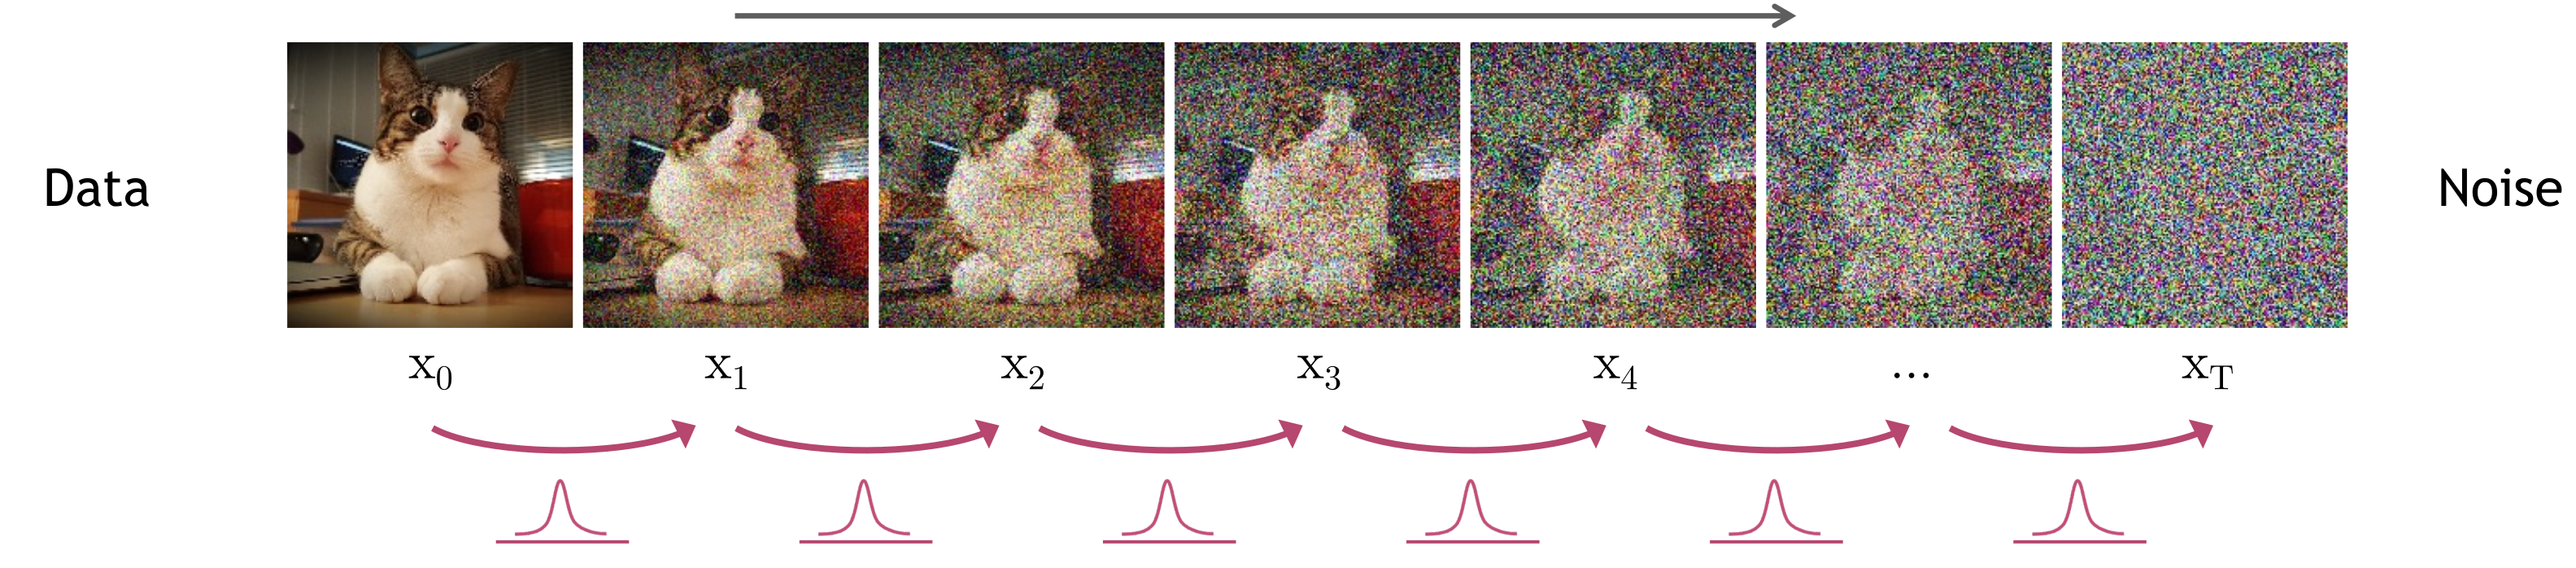
\includegraphics[width=0.7\textwidth]{images/forward.png}
        \caption{CVPR 2022 tutorial}
    \end{figure}
    \note{
     - leave room for obvious question: just set $\beta_i=1$?
     - same domain
    }
\end{frame}

\begin{frame}
    \frametitle{Generative Process}
    Let $q(\bm{x}^{0})$ be data distribution. Given that Markov chain, how to sample from $p(\bm{x}^{0} | \bm{x}^{T})$? Note that the forward is fixed, conditional $q(\bm{x}^{t}| \bm{x}^{t-1})$ is known, $q(\bm{x}^{T}) \approx \mathcal{N}(\bm{x}^{T}| \bm{0}, \bm{I})$ .
    \begin{figure}
        \centering
        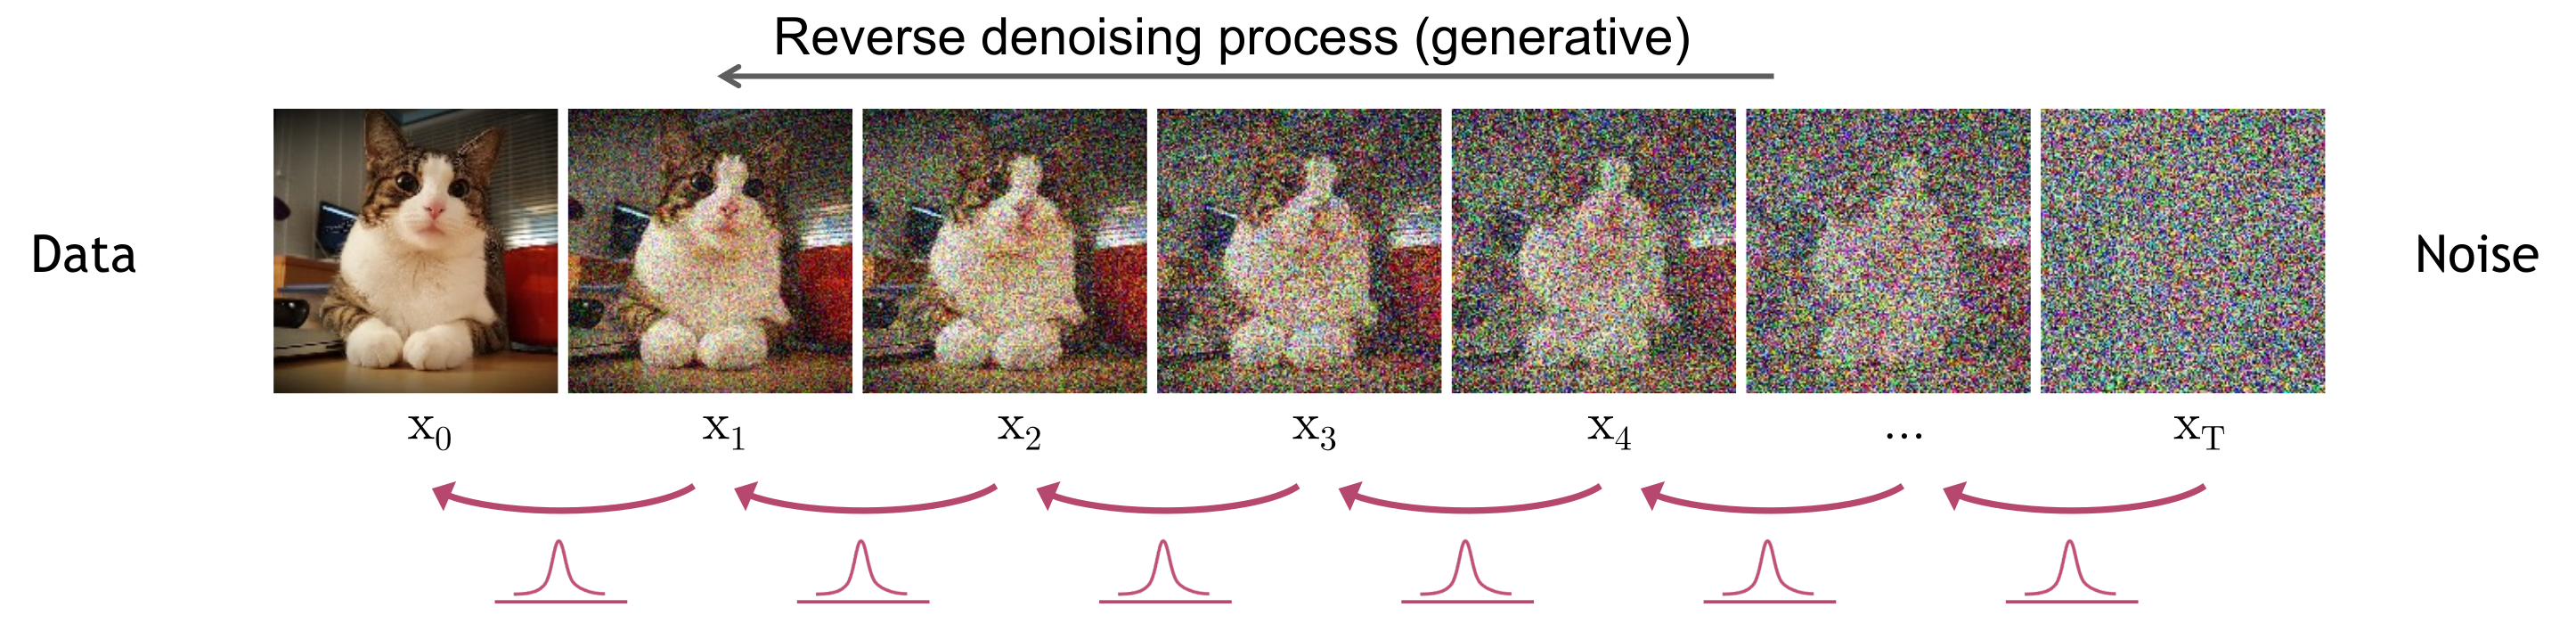
\includegraphics[width=0.7\textwidth]{images/backward.png}
        \caption{CVPR 2022 tutorial}
    \end{figure}

    A naive but sound strategy:
    \begin{itemize}
        \item Sample $\bm{x}^{T} \sim \mathcal{N}(\bm{x}^{T}| \bm{0}, \bm{I})$
        \item Sample $\bm{x}^{t-1} \sim p(\bm{x}^{t-1}| \bm{x}^{t}) \propto p(\bm{x}^{t-1}, \bm{x}^{t}) = q(\bm{x}^t | \bm{x}^{t-1}) p(\bm{x}^{t-1}) $ $\Rightarrow$ intractable. 

    \end{itemize}
        Good news is if $\beta_t$ in 
        $ q(\bm{x}^{t}|\bm{x}^{t-1}) \triangleq \mathcal{N}(\bm{x}^{t}; \bm{x}^{t-1}\sqrt{1-\beta_t}, \beta_t \bm{I})$ 
        is small enough, then 
        $p(\bm{x}^{t-1}| \bm{x}^{1})$ is also a normal distribution.
\end{frame}

\begin{frame}
    \frametitle{Recipe}
    \begin{itemize}
        \item Let $q(\bm{x}^{0})$ denote the unknown data distribution
        \item Define $\beta_t, 1\leq t \leq T$ such that
            \begin{align}
                &q(\bm{x}^{t}|\bm{x}^{t-1}) \triangleq \mathcal{N}(\bm{x}^{t}; \bm{x}^{t-1}\sqrt{1-\beta_t}, \beta_t \bm{I}), \quad 0\leq \beta_t \leq 1 \\
                &q(\bm{x}^{T} | \bm{x}^{0}) \; \; \approx \mathcal{N}(\bm{x}^{T}; \bm{0}, \bm{I})  \\
                &p(\bm{x}^{t-1}| \bm{x}^{t}) \text{ is normal} \quad \; \forall 1\leq t \leq T
            \end{align} 
            Since we know $p(\bm{x}^{t-1}|\bm{x}^{t})$ is normal, it can be parameterized as
            \[
            p(\bm{x}^{t-1}| \bm{x}^{t}) \sim \mathcal{N}(\bm{x}^{t-1}; \boldsymbol \mu_{\theta}(\bm{x}^{t}, t), \sigma^2 \bm{I})
            \] 
    \end{itemize}
    \begin{figure}
        \centering
        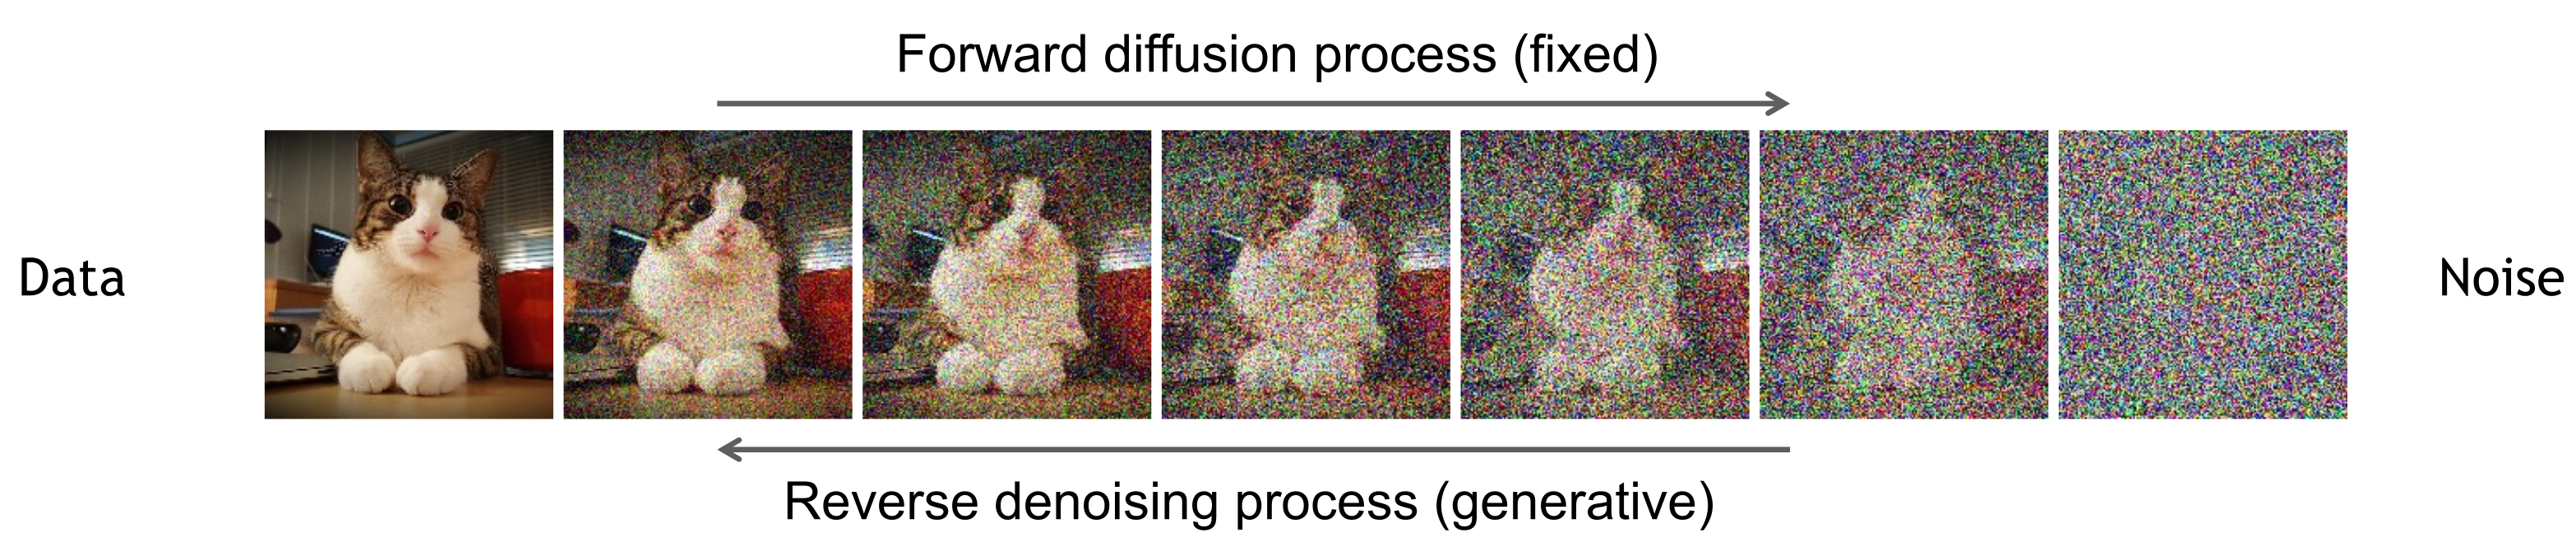
\includegraphics[width=0.7\textwidth]{images/bidirection.png}
        \caption{CVPR 2022 tutorial}
    \end{figure}
    {\red There is no assumption on data distribution}
\end{frame}

\begin{frame}
    \frametitle{Training}
    \begin{itemize}
        \item Latent variables $\bm{x}^{1\ldots T}$
        \item Model probability  $p(\bm{x}^{0}) = \int p(\bm{x}^{0\ldots T}) d\bm{x}^{1\ldots T}$
        \item Data distribution $q(\bm{x}^{0})$
        \item Posterior probability $q(\bm{x}^{1\ldots T} | \bm{x}^{0})$
    \end{itemize}
    % Using MLE principle, 
    We try to minimize KL divergence between model probability and the real data distribution (which reduces to MLE), 
    % which leads to
    \[
    \maximize_{\bm{x}^{1\ldots T}}\; \mathop{\mathbb{E}}_{\bm{x} \sim q(\bm{x}^{0})} \log p(\bm{x}^{0})
    \] 
    \begin{align*}
    p(\bm{x}^{0})
    &= \int p(\bm{x}^{0\ldots T}) \dfrac{q(\bm{x}^{1\ldots T}|\bm{x}^{0})}{q(\bm{x}^{1\ldots T}|\bm{x}^{0})} d \bm{x}^{1\ldots T}\\
    &= \int q(\bm{x}^{1\ldots T}|\bm{x}^{0}) \dfrac{p(\bm{x}^{0\ldots T})}{q(\bm{x}^{1\ldots T}|\bm{x}^{0})} d \bm{x}^{1\ldots T}\\
    &= \int q(\bm{x}^{1\ldots T}|\bm{x}^{0}) p(\bm{x}^{T}) \prod_{i=1}^{T}\dfrac{p(\bm{x}^{t-1}| \bm{x}^{t})}{q(\bm{x}^{t}|\bm{x}^{t-1})} d \bm{x}^{1\ldots T} \\
    &= \mathop{\mathbb{E}}_{q(\bm{x}^{1\ldots T}|\bm{x}^{0})} \left[  p(\bm{x}^{T}) \prod_{i=1}^{T}\dfrac{p(\bm{x}^{t-1}| \bm{x}^{t})}{q(\bm{x}^{t}|\bm{x}^{t-1})} \right]
    \end{align*}
    % \begin{align*}
    %     L &= \mathop{\mathbb{E}}_{q(\bm{x}^{0})} \left[ \log p(\bm{x}^{0}) \right] \\
    %       &= 
    % \end{align*}
\end{frame}

\begin{frame}
    \frametitle{Training}
    What we want
    \[
    \maximize_{\bm{x}^{1\ldots T}}\; \mathop{\mathbb{E}}_{\bm{x} \sim q(\bm{x}^{0})} \log p(\bm{x}^{0})
    \] 
    What we know is
    \begin{align*}
    \mathop{\mathbb{E}}_{\bm{x} \sim q(\bm{x}^{0})} \log p(\bm{x}^{0})
    &= \mathop{\mathbb{E}}_{q(\bm{x}^{0})} \log \left( \mathop{\mathbb{E}}_{q(\bm{x}^{1\ldots T}|\bm{x}^{0})} \left[  p(\bm{x}^{T}) \prod_{i=1}^{T}\dfrac{p(\bm{x}^{t-1}| \bm{x}^{t})}{q(\bm{x}^{t}|\bm{x}^{t-1})} \right]
 \right) \\
    &\geq \mathop{\mathbb{E}}_{q(\bm{x}^{0\ldots T})} \log \left[  p(\bm{x}^{T}) \prod_{i=1}^{T}\dfrac{p(\bm{x}^{t-1}| \bm{x}^{t})}{q(\bm{x}^{t}|\bm{x}^{t-1})} \right]
    \end{align*}
    % which can be shown be lower bounded by $K =\ldots $
\end{frame}

% \begin{frame}
%     \frametitle{Score matching for estimating un-normalized probability model}
%     % \begin{itemize}
%     %     \item Whenever using MLE principle, it is required to work with normalized probability model (proper pdf)
%     %     \item But it is usually the case that computing normalization factor is intractable
%     %     \item In some cases, learning un-normalized probability model is sufficient.
%     % \end{itemize}
%     Setting:
%     \begin{itemize}
%         \item Let $f(\bm{x}; \theta)$ be an parameterized un-normalized probability model
%         \item The corresponding normalization factor $Z(\boldsymbol \theta)$
%         \item The proper pdf is $\widetilde{f}(\bm{x}) = f(\bm{x}; \boldsymbol \theta) / Z(\boldsymbol \theta)$
%         \item Let $s_{\boldsymbol \theta}(\bm{x}) \triangleq \nabla_{\bm{x}} \log \widetilde{f}(\bm{x}; \boldsymbol \theta) = \nabla_{\bm{x}} (\log f(\bm{x}; \boldsymbol \theta) - \log Z(\boldsymbol \theta)) = \nabla_{\bm{x}} \log f(\bm{x}; \boldsymbol \theta)$ (Stein score)
%     \end{itemize}
% \end{frame}

\begin{frame}
    \frametitle{Estimate un-normalized probability model }
    Problem setting:
    \begin{itemize}
        \item $\bm{x}_1, \ldots , \bm{x}_N \in \mathbb{R}^{n}$ are drawn i.i.d from $p_{\text{data}}(\bm{x})$.
        \item Assume we know that $p_{\text{data}}$ belong a distribution class $p_{\boldsymbol \theta}(\bm{x}) = q(\bm{x}; \boldsymbol \theta)/ Z(\boldsymbol \theta)$.
        \item Functional form of $q(\bm{x}; \boldsymbol \theta)$ is known, but $Z(\boldsymbol \theta) = \int_{\bm{x}} q(\bm{x}; \boldsymbol \theta) d\bm{x}$ is intractable.
        \item Goal: We want to use $\bm{x}_i$'s to estimate $\boldsymbol \theta_{\text{data}}$ corresponding to $p_{\text{data}}$ (assume it is unique).
    \end{itemize}
\parencite{hyvarinen2005estimation} proposed to
    \begin{equation}
        \minimize_{\boldsymbol \theta} \; \mathop{\mathbb{E}}_{p_{\text{data}}} \left[  \norm{\nabla_{\bm{x}} \log p_{\boldsymbol \theta}(\bm{x}) - \nabla_{\bm{x}} \log p_{\text{data}}(\bm{x})}^2\right]
    \end{equation}
\begin{itemize}
    \item Normalization factor plays no role here. $\nabla_{\bm{x}} \log p_{\boldsymbol \theta}(\bm{x}) = \nabla_{\bm{x}}(\log q(\bm{x}; \boldsymbol \theta) - \log Z(\boldsymbol \theta)) = \nabla_{\bm{x}} \log q(\bm{x}; \boldsymbol \theta)$.
    \item (1)  is surprisingly equivalent to 
    \begin{equation*}
        \minimize_{\boldsymbol \theta} \; \mathop{\mathbb{E}}_{p_{\text{data}}} \left[ \text{tr}(\nabla_{\bm{x}} \bm{s}_{\boldsymbol \theta}(\bm{x})) + \dfrac{1}{2} \norm{\bm{s}_{\boldsymbol \theta}(\bm{x})}^2\right]
    \end{equation*}
    where the so-cal {\blue score} $\bm{s}_{\boldsymbol \theta}(\bm{x})\triangleq \nabla_{\bm{x}} q(\bm{x}; \boldsymbol \theta)$.
\end{itemize}
\end{frame}


\begin{frame}
    \frametitle{Generative Modeling by Estimating Gradients of the Data Distribution}
    General recipe include 2 ingredients:
    \begin{itemize}
        \item Step 1: Using score match to estimate score of data distribution.
        \item Step 2: Using Langevin dynamics to draw samples using score function.
            \[
            \bm{x}_t = \bm{x}_{t-1} + \dfrac{\epsilon}{2} \nabla_{\bm{x}} \log p(\bm{x}_{t-1}) + \sqrt{\epsilon} \bm{z}_t,
            \] 
            where $\bm{z}_t \sim \mathcal{N}(0, \bm{I}), \bm{x}_0 \sim \pi(\bm{x})$. This would produce $\bm{x}_{t} \sim p(\bm{x})$ when $\epsilon \to 0, t \to \infty$ (in practice, $T=100, \epsilon = 2e^{-5}$ ).
    \end{itemize}

\end{frame}

\begin{frame}
    \frametitle{Generative Modeling by Estimating Gradients of the Data Distribution}
    % General recipe include 2 ingredients:
    % \begin{itemize}
    %     \item Step 1: Using score match to estimate score of data distribution.
    %     \item Step 2: Using Langevin dynamics to draw samples using score function.
    % \end{itemize}

    Challenges in step 1: computation complexity
    \begin{equation*}
        \minimize_{\boldsymbol \theta} \; \mathop{\mathbb{E}}_{p_{\text{data}}} \left[ \text{tr}(\nabla_{\bm{x}} \bm{s}_{\boldsymbol \theta}(\bm{x})) + \dfrac{1}{2} \norm{\bm{s}_{\boldsymbol \theta}(\bm{x})}^2\right]
    \end{equation*}
    \begin{itemize}
        \item Computing the first term $\text{tr}(\cdot)$ (involving Jacobian) is costly for high dimensional data.
            \begin{itemize}
                \item Solution 1 \parencite{vincent2011connection}. Add pre-specified noise to data $q_{\sigma}(\widetilde{\bm{x}}| \bm{x})$, then using score matching to learn score of $q_{\sigma}(\bm{x}) = \int_{\bm{x}} q_{\sigma}(\widetilde{\bm{x}}| \bm{x}) p_{\text{data}}(\bm{x}) d \bm{x}$ (instead of $p_{\text{data}}$ ).

                    It was shown that the objective is equivalent to
                    \[
                    \mathop{\mathbb{E}}_{\widetilde{\bm{x}} \sim q_{\sigma}(\cdot)} \left[ \norm{\bm{s}_{\theta}(\widetilde{\bm{x}}) - \nabla_{\widetilde{\bm{x}}} \log q_{\sigma}(\widetilde{\bm{x}}| \bm{x})}^2 \right],
                    \] 
                    and by score matching's result, the optimal solution $\bm{s}_{\boldsymbol \theta^{\star }} (\bm{x}) = \nabla_{\bm{x}} \log q_{\sigma}(\bm{x}) \approx p_{\text{data}}(\bm{x})$.

            \end{itemize}
    \end{itemize}
\end{frame}

\begin{frame}
    \begin{itemize}
        \item Solution 2: \parencite{song2020sliced} Random projection to estimate $\text{tr}(\cdot)$. The objective now become
            \[
            \mathop{\mathbb{E}}_{p_{\bm{v}}} \mathop{\mathbb{E}}_{p_{\text{data}}} \left[ \bm{v}^{\T} (\nabla_{\bm{x}} \bm{s}_{\boldsymbol \theta}(\bm{x})) \bm{v} + \dfrac{1}{2} \norm{\bm{s}_{\boldsymbol \theta}(\bm{x})}^2\right]
            \] 
    \end{itemize}
    Several other challenges are demonstrated in \parencite{song2020score}. In the end, they proposed to add noise with different variance.
    \begin{figure}
        \centering
        \begin{subfigure}{0.50\textwidth}
            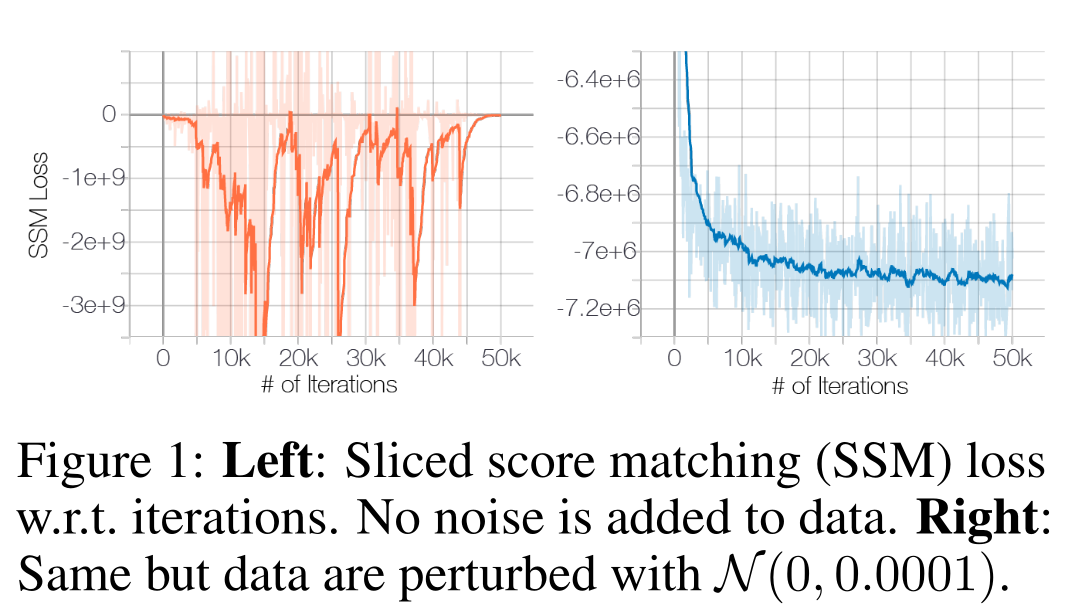
\includegraphics[width=\textwidth,trim={0 6.2cm 0 0},clip]{images/manifold.png}
            \caption{Low dimension manifold. Left: train with original MNIST, right: add noise $\mathcal{N}(0, 0.0001)$ }
        \end{subfigure}
        \begin{subfigure}{0.35\textwidth}
            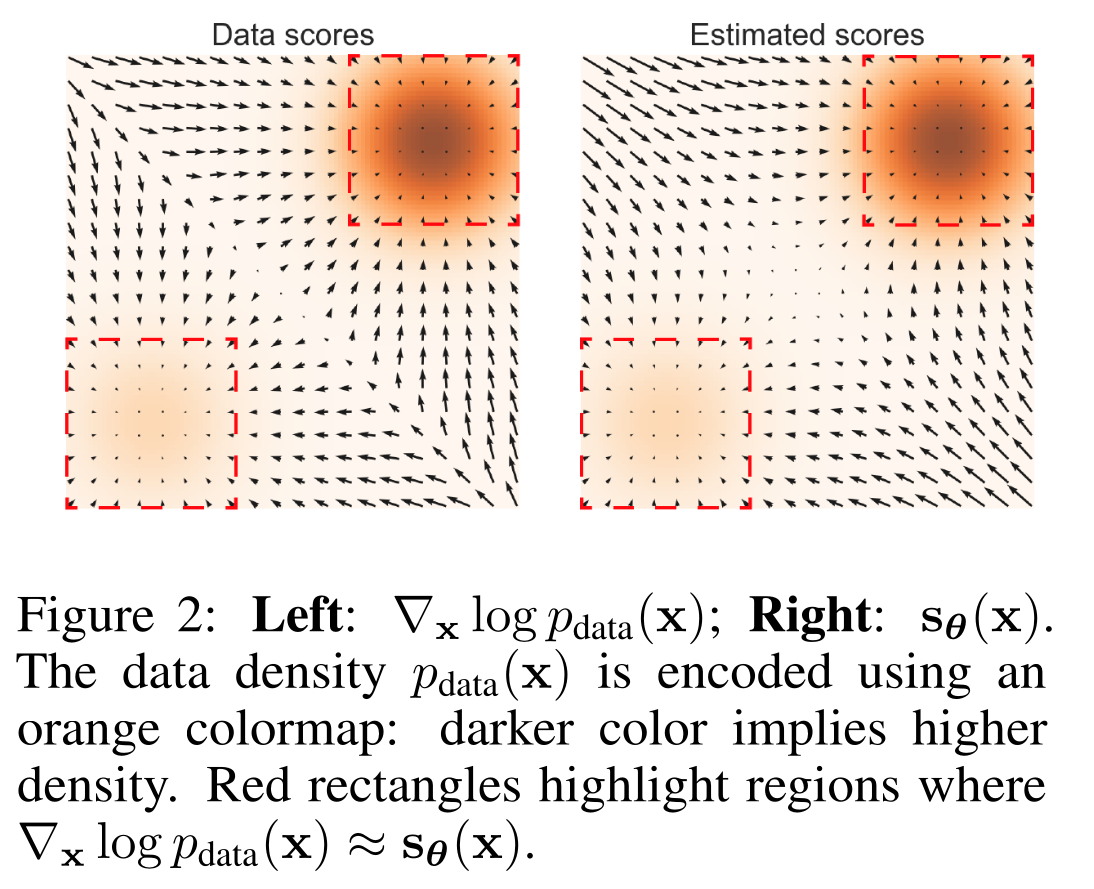
\includegraphics[width=\textwidth,trim={0 11cm 0 0},clip]{images/inaccurate_score.png}
            \caption{In low density region, there is not enough data to learn $\nabla_{\bm{x}} \log p_{\text{data}}$ }
        \end{subfigure}
    \end{figure}
\end{frame}

\begin{frame}
    \frametitle{Suggestion if anyone's interested}
    \begin{itemize}
        \item \fullcite{ho2020denoising}
        \item \fullcite{song2020score}
    \end{itemize}
    
\end{frame}

% \begin{frame}
%     Very useful resources:
%     \begin{itemize} 
%         \item Slide from ICLR 2020?
%     \end{itemize}
% \end{frame}
%
% \begin{frame}
%     \frametitle{todo}
%     \begin{itemize}
%         \item consider using $P$ instead of $p$
%         \item the leading to diffusion is still not clear
%     \end{itemize}
% \end{frame}

\end{document}
